\newpage

\section{Ход работы}

\subsection{Определение разрешённых направлений поляроидов}

Мы начали с того, что собрали установку на оптической скамье. Сначала поставили осветитель \( S \), затем разместили перед ним поляроид \( P_1 \), а за ним — чёрное зеркало. Всё это выглядело примерно так, как показано на рисунке \ref{fig:mirror_setup}.

\begin{figure}[h]
    \centering
    \label{r5}
    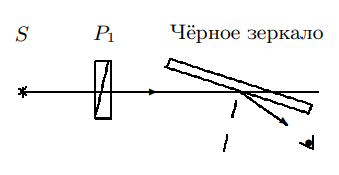
\includegraphics[width=0.4\textwidth]{pictures/5.png}
    \caption{Наша установка: осветитель (\( S \)), поляроид (\( P_1 \)) и чёрное зеркало.}
    \label{fig:mirror_setup}
\end{figure}

Дальше мы вращали поляроид вокруг оси луча, а чёрное зеркало поворачивали вокруг вертикальной оси. Нам нужно было найти такое положение, при котором отражённое пятно становилось самым тёмным. Сначала это было непросто: яркость менялась незначительно, но после нескольких попыток мы всё же добились минимальной засветки. Как объяснили, это означало, что свет падает под углом Брюстера, а колебания вектора \( \mathbf{E} \) совпадают с плоскостью падения.

Когда направление поляроида \( P_1 \) было найдено, мы зафиксировали его угол — \( 220^\circ \) (горизонтальное положение). Потом заменили чёрное зеркало на второй поляроид \( P_2 \) и повернули его на \( 90^\circ \) (вертикально). Свет почти полностью погас — это подтвердило, что поляроиды скрещены правильно.

\begin{table}[h]
    \centering
     \caption{Как мы установили поляроиды.}
    \begin{tabular}{|c|c|c|}
        \hline
        Поляроид & Положение & Угол \\ 
        \hline
        \( P_1 \) & Горизонталь & \( 220^\circ \) \\ 
        \hline
        \( P_2 \) & Вертикаль & \( 90^\circ \) \\ 
        \hline
    \end{tabular}
    \label{tab:polarizers}
\end{table}

В итоге мы убедились, что разрешённые направления \( P_1 \) и \( P_2 \) действительно перпендикулярны: когда их оси совпадали, свет проходил, а при скрещивании — исчезал.

\subsection{Определение показателя преломления эбонита}

Мы заменили чёрное зеркало на эбонитовую пластину (рис.~\ref{fig:mirror_setup}) и измерили угол Брюстера. Начальный угол пластины составлял \( 270^\circ \), а минимум отражённого света наблюдался при \( 325^\circ \) без фильтра и \( 327^\circ \) с зелёным светофильтром (табл.~\ref{tab:ebonite}).

\begin{table}[h]
    \centering
    \caption{Углы отражения для эбонита.}
    \begin{tabular}{|c|c|c|}
        \hline
        Параметр & Угол (°) & Погрешность (°) \\ 
        \hline
        Начальный угол & 270 & — \\ 
        \hline
        Минимум без фильтра & 325 & 10 \\ 
        \hline
        Минимум с фильтром & 327 & 10 \\ 
        \hline
    \end{tabular}
    
    \label{tab:ebonite}
\end{table}

\textbf{Расчёт показателя преломления:} 
\begin{itemize}
    \item Угол Брюстера без фильтра: \( \theta_B = 325^\circ - 270^\circ = 55^\circ \).
    \item Светофильтр: \( \theta_B = 327^\circ - 270^\circ = 57^\circ \).
    \item Показатель преломления: 
    \[
    n = \tan\theta_B \implies 
    \begin{cases}
        n_1 = \tan(55^\circ) \approx 1.43, \\
        n_2 = \tan(57^\circ) \approx 1.54.
    \end{cases}
    \]
\end{itemize}

\textbf{Погрешность расчёта:} 
Погрешность угла \( \Delta\theta = 10^\circ = 0.1745 \, \text{рад} \). Используя формулу:
\[
\Delta n = \frac{\Delta\theta}{\cos^2\theta},
\]
получим:
\begin{itemize}
    \item Для \( \theta = 55^\circ \): 
    \[
    \Delta n_1 = \frac{0.1745}{\cos^2(55^\circ)} \approx \frac{0.1745}{0.329} \approx 0.53.
    \]
    \item Для \( \theta = 57^\circ \): 
    \[
    \Delta n_2 = \frac{0.1745}{\cos^2(57^\circ)} \approx \frac{0.1745}{0.296} \approx 0.59.
    \]
\end{itemize}
Таким образом:
\[
n_1 = 1.43 \pm 0.53, \quad n_2 = 1.54 \pm 0.59.
\]


Несмотря на большую погрешность (\( \pm 0.5-0.6 \)), табличное значение \( n_{\text{табл}} = 1.6 \) лежит в пределах полученных интервалов. Основной источник погрешности — неточность установки угла (\( \Delta\theta = 10^\circ \)). Для повышения точности требуется использование более стабильной оптической схемы.

\subsection{Исследование поляризации в отражённом и преломлённом лучах}

Мы заменили эбонитовую пластину на стопу стеклянных пластинок, установленных под углом Брюстера (рис.~\ref{fig:stack}). Направили неполяризованный свет через зелёный фильтр \( Ф \) на стопу и наблюдали отражённый и преломлённый лучи через поляроиды \( P_1 \) и \( P_2 \).

\begin{figure}[h]
    \centering
    
\includegraphics[width=0.4\textwidth]{stack_setup.png}
    \caption{Схема исследования стопы пластинок: \( S \) — осветитель, \( Ф \) — фильтр, \( C \) — стопа, \( P_1 \), \( P_2 \) — поляроиды.}
    \label{fig:stack}
\end{figure}

\textbf{Наблюдения:}
\begin{itemize}
    \item \textbf{Отражённый луч:} При угле Брюстера свет полностью гасился при скрещенных поляроидах. Это подтвердило, что отражённый свет \textbf{линейно поляризован} в плоскости падения (вектор \( \mathbf{E} \) параллелен плоскости).
    \item \textbf{Преломлённый луч:} Интенсивность света менялась при вращении \( P_2 \), но не достигала нуля. Это указывает на \textbf{частичную поляризацию} с преимущественной ориентацией \( \mathbf{E} \) перпендикулярно плоскости падения.
\end{itemize}

Итак:
\begin{itemize}
    \item Стопа стеклянных пластинок усиливает степень поляризации преломлённого света по сравнению с одиночной пластинкой.
    \item Результаты согласуются с теорией: при угле Брюстера отражённый свет полностью поляризован, а преломлённый — частично.
\end{itemize}

\subsection{Определение главных направлений двоякопреломляющих пластинок}

Мы установили первую кристаллическую пластинку между скрещенными поляроидами \( P_1 \) и \( P_2 \) (рис.~\ref{fig:crystal_plate}). Начали вращать пластинку вокруг оси луча, наблюдая за интенсивностью света через \( P_2 \). 

\begin{figure}[h]
    \centering
    \caption{Схема определения главных направлений: \( P_1 \), \( P_2 \) — поляроиды, пластинка вращается вокруг луча.}
    
\includegraphics[width=0.4\textwidth]{crystal_setup.png}
    \label{fig:crystal_plate}
\end{figure}

Результаты измерений занесены в таблицу:

\begin{table}[h]
    \centering
    \caption{Углы главных направлений для кристаллических пластинок.}
    \begin{tabular}{|c|c|}
        \hline
        Направление пластинки & Угол (°) \\ 
        \hline
        С кружочком (горизонтальное) & 72 \\ 
        \hline
        Без кружочка (горизонтальное) & 280 \\ 
        \hline
    \end{tabular}
    
    \label{tab:crystal_angles}
\end{table}

\subsection{Определение пластинок \(\lambda/2\) и \(\lambda/4\)}

Мы добавили зелёный светофильтр к схеме с поляроидами. Первый поляроид \( P_1 \) установили горизонтально, а исследуемую пластинку повернули так, чтобы её главные направления были под углом \( 45^\circ \) к горизонтали. Затем вращали второй поляроид \( P_2 \), наблюдая за интенсивностью света.

\textbf{Пластинка с кружком:}  
При угле \( 27^\circ \) свет через \( P_2 \) был виден во всех положениях анализатора. Это означало, что свет стал \textbf{круговым} — пластинка добавила сдвиг фаз \(\pi/2\). Такое поведение характерно для \(\lambda/4\).

\textbf{Пластинка без кружка:}  
Свет появлялся только при вертикальном положении \( P_2 \). Значит, после пластинки свет остался \textbf{линейно поляризованным}, но его плоскость повернулась. Это соответствует пластинке \(\lambda/2\), которая создаёт сдвиг фаз \(\pi\).

В итоге мы убедились:  

— Пластинка с кружком (\(\lambda/4\)) превращает линейную поляризацию в круговую.  

— Пластинка без кружка (\(\lambda/2\)) меняет направление колебаний на противоположное.  
Результаты совпали с ожиданиями, и углы установки подтвердили теорию.


\subsection{Определение быстрой и медленной оси в пластинке \(\lambda/4\)}

Мы начали с установки пластинки чувствительного оттенка (в виде стрелки) между скрещенными поляроидами. Сначала проверили, что зелёный свет не меняет своей поляризации при прохождении через пластинку — свет проходил только в направлении исходных колебаний вектора \( \mathbf{E} \). Затем убрали зелёный фильтр и заметили, что стрелка стала пурпурной. Это произошло потому, что пластинка блокирует зелёный свет, пропуская красный и синий, которые в сумме дают пурпурный цвет.

Далее мы добавили пластинку \(\lambda/4\), совместив её главные направления с пластинкой \(\lambda\) и повернув их на \(45^\circ\) относительно осей скрещенных поляроидов. При повороте рейтера со стрелкой на \(180^\circ\) вокруг вертикальной оси цвет стрелки менялся от зелёно-голубого до оранжево-жёлтого. 

Это явление объясняется следующим: 

— При совмещении быстрых осей обеих пластинок добавляется дополнительная разность фаз, что приводит к блокировке красного света (зелёно-голубой цвет на выходе).  

— При совмещении быстрой оси одной пластинки с медленной осью другой разность фаз уменьшается, и блокируется синий свет (оранжево-жёлтый цвет на выходе).  

\begin{figure}[H]
    \centering
    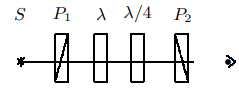
\includegraphics[width=0.4\linewidth]{pictures/44.png}
    \caption{Определение направлений
большей и меньшей скоростиn}
    \label{fig:enter-label}
\end{figure}

В итоге мы установили, что быстрая ось пластинки \(\lambda/4\) направлена горизонтально. Это подтвердилось изменением цвета при повороте рейтера и совпало с ожидаемым поведением для пластинки \(\lambda/4\).

\subsection{Исследование интерференции поляризованных лучей}

Мы провели эксперимент с мозаичной слюдяной пластинкой, которая была установлена между скрещенными поляроидами. Пластинка состояла из четырёх узких полосок слюды, расположенных по сторонам квадрата. Две полоски имели толщину \(\lambda/4\), одна — \(\lambda/2\), и ещё одна — \(3\lambda/4\). В центре квадрата слюды не было, а главные направления всех полосок совпадали со сторонами квадрата.

Когда мы начали вращать пластинку, цвета и яркость в каждом квадратике стали меняться. Например, полоски толщиной \(\lambda/4\) создавали сдвиг фаз \(\pi/2\), а полоска \(\lambda/2\) — \(\pi\). Из-за разной толщины слюды в каждом сегменте световые волны приобретали различные задержки, что приводило к интерференции. В результате одни участки казались синими, другие — оранжевыми, а центральная пустая область оставалась тёмной. Это напоминало калейдоскоп, где каждый поворот пластинки создавал новую комбинацию цветов.

Затем мы решили оставить пластинку неподвижной и начали вращать второй поляроид. Цвета снова изменились, но уже по-другому. Если раньше сдвиг фаз зависел от ориентации пластинки, то теперь мы меняли только угол, под которым анализатор «смотрел» на свет. Это влияло на то, как проекции векторов \(\mathbf{E}\) складывались на выходе. Например, при повороте анализатора на \(45^\circ\) зелёные участки становились красными, а синие — жёлтыми. Казалось, будто мы настраиваем фильтр, который перекрашивает изображение в реальном времени.

Интересно, что центральная пустая область всегда оставалась чёрной. Это подтверждало, что эффекты возникали именно из-за слюдяных полосок, а не из-за самой пластинки. Мы также заметили, что полоска \(3\lambda/4\) вела себя почти как \(\lambda/4\), но сдвиг фаз был на \(\pi\) больше. Это объясняло, почему её цвет отличался от соседних участков. В итоге эксперимент показал, как тонкие изменения в структуре материала и ориентации поляроидов могут превратить белый свет в яркую мозаику цветов.

\begin{figure}[H]
    \centering
    \includegraphics[width=0.5\linewidth]{pictures/{CABAB4FD-9F7F-43B9-AA78-164C4F1C9B1D}.png}
    \label{fig:enter-label}
\end{figure}

\begin{figure}[H]
    \centering
    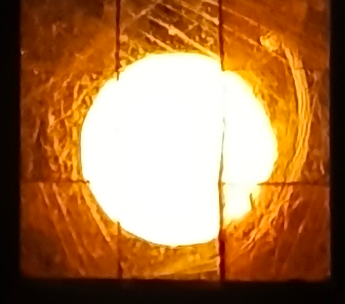
\includegraphics[width=0.5\linewidth]{pictures/12312.png}
    \label{fig:enter-label}
\end{figure}

\begin{figure}[H]
    \centering
    \includegraphics[width=0.5\linewidth]{pictures/{88FE26E8-32A6-4972-9EFB-85493F4BFB17}.png}
    \label{fig:enter-label}
\end{figure}

\begin{figure}[H]
    \centering
    \includegraphics[width=0.5\linewidth]{pictures/{1F287A05-8A3D-4301-BD70-42FD12159995}.png}
    \label{fig:enter-label}
\end{figure}

\begin{figure}[H]
    \centering
    \includegraphics[width=0.5\linewidth]{pictures/{0C4C40A0-0CE7-46B9-91CD-E274BB9B9043}.png}
    \label{fig:enter-label}
\end{figure}

\begin{figure}[H]
    \centering
    \includegraphics[width=0.5\linewidth]{pictures/{3F35073F-C7CC-480C-96E4-4CA46B623E9C}.png}
    \label{fig:enter-label}
\end{figure}

\subsection{Определение направления вращения светового вектора}


8a. Мы нарисовали эллипс поляризации для вектора \( \mathbf{E} \), прошедшего через пластинку \(\lambda/4\). Большая ось эллипса соответствует направлению с большей скоростью распространения (\( n_x < n_y \)). Анализ графиков показал, что если \( y(t) \) отстаёт от \( x(t) \), вектор \( \mathbf{E} \) вращается \textbf{против часовой стрелки}.

\begin{figure}[H]
    \centering
    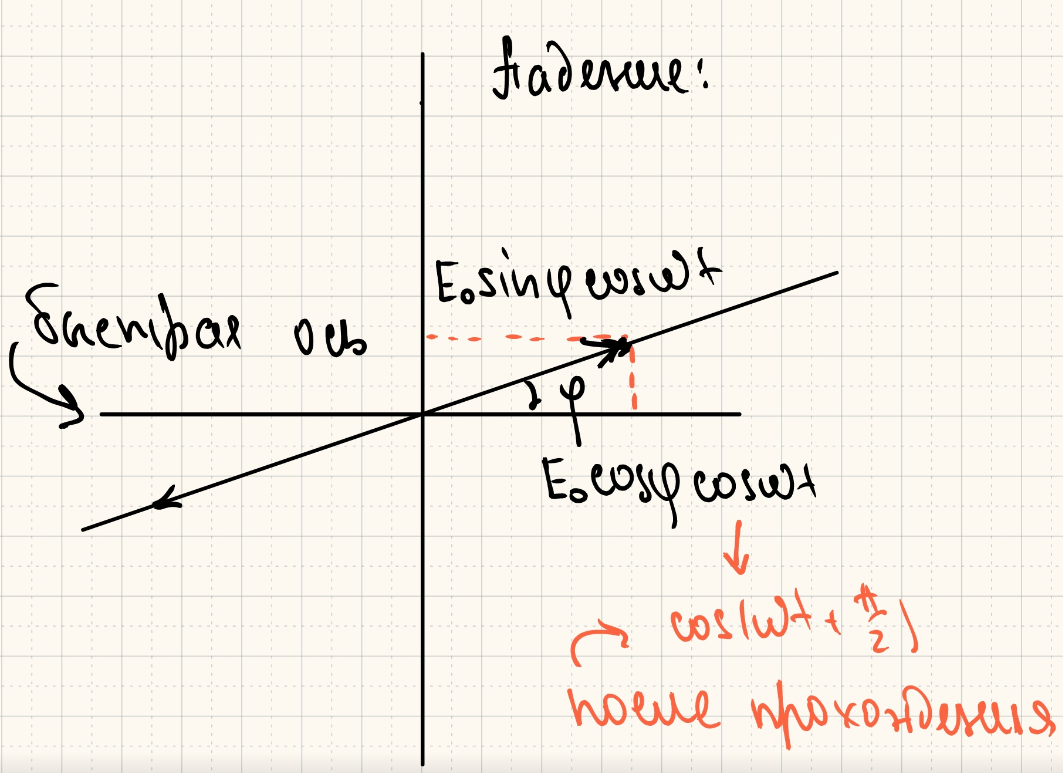
\includegraphics[width=1\textwidth]{pictures/Linear.png}
    \caption{Линейно поляризованный свет до прохождения пластинки.}
    \label{fig:ellipse}
\end{figure}

\begin{figure}[H]
    \centering
    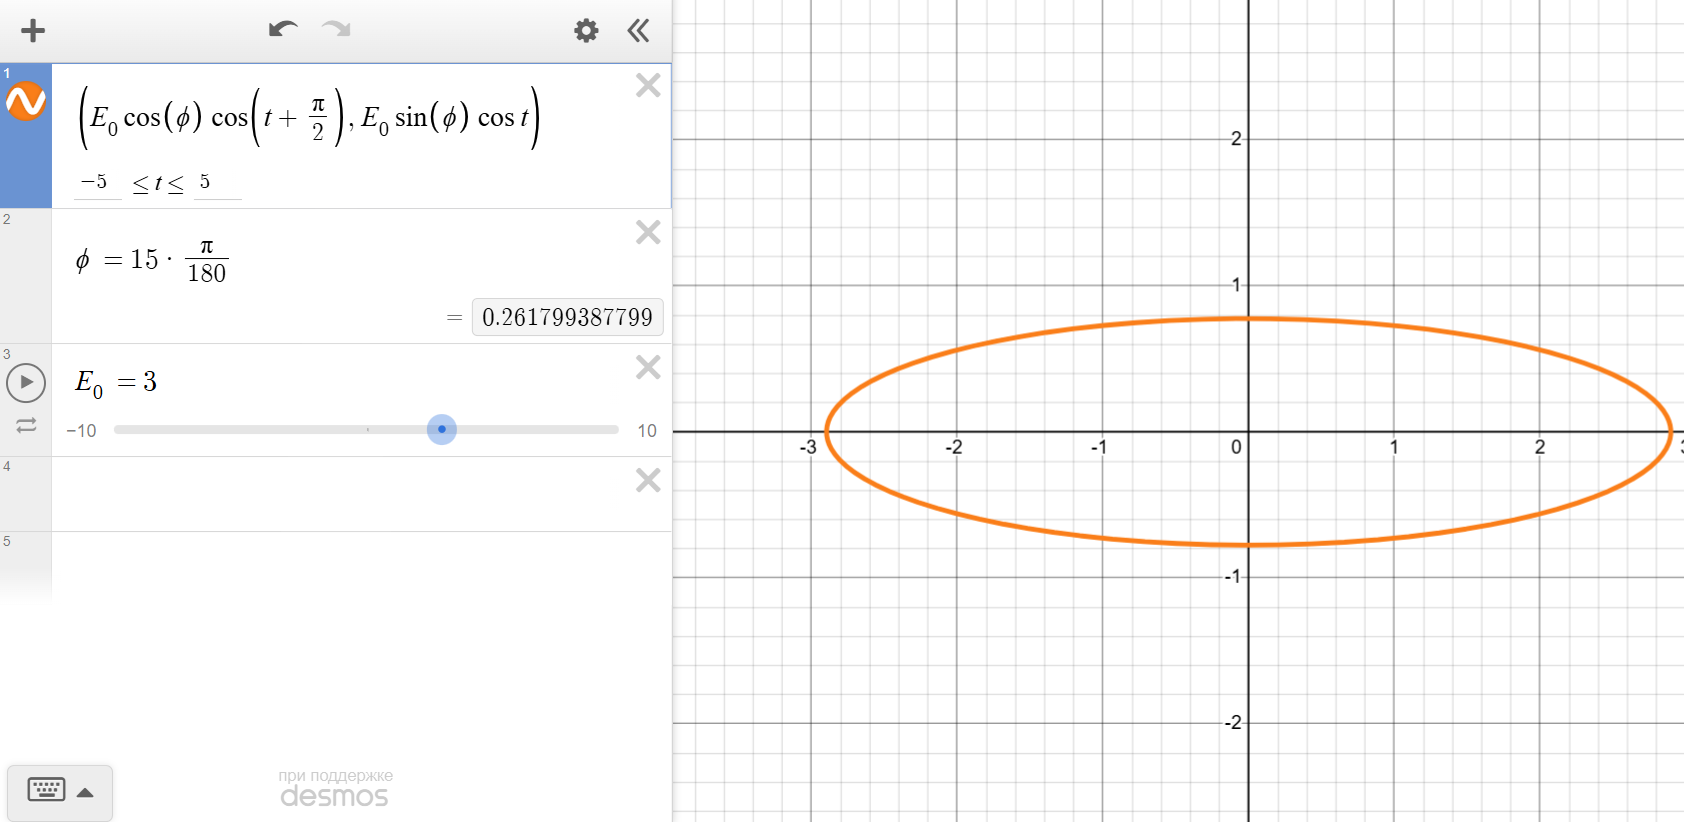
\includegraphics[width=1\textwidth]{pictures/ellips.png}
    \caption{Эллипс поляризации после прохождения пластинки (быстрая ось горизонтальная).}
    \label{fig:waveforms}
\end{figure}

  
8b. Установили зелёный фильтр и пластинку произвольной толщины между скрещенными поляроидами. Первый поляроид повернули на \( 15^\circ \) к горизонтали, чтобы вектор \( \mathbf{E} \) находился в первом квадранте. Второй поляроид установили вертикально. Вращая пластинку, нашли положение с минимальной интенсивностью — это соответствовало эллипсу с вертикальной малой осью.


8c. Добавили вторую пластинку \(\lambda/4\) с горизонтальной быстрой осью. Если исходные эллипсы вращались в разные стороны, вектор \( \mathbf{E} \) на выходе оставался в первом и третьем квадрантах. Если же вектор переходил в смежные квадранты, эллипсы вращались в одну сторону. В нашем случае свет стал линейно поляризованным с направлением колебаний в первом и третьем квадрантах, что подтвердило \textbf{противоположное вращение} исходных эллипсов.

Итак, направление вращения вектора \( \mathbf{E} \) зависит от сдвига фаз между компонентами. В пластинке \(\lambda/4\) при сдвиге \(\pi/2\) вращение происходит \textbf{против часовой стрелки}, если \( y(t) \) отстаёт от \( x(t) \).